\documentclass[11pt,a4paper]{article}
\usepackage[utf8]{inputenc}
\usepackage[spanish,es-nodecimaldot]{babel}
\usepackage{amsmath,amssymb,amsfonts}
\usepackage{geometry}
\geometry{margin=2.5cm}
\usepackage{graphicx}
\usepackage{booktabs}
\usepackage{hyperref}
\usepackage{listings}
\usepackage{xcolor}
\usepackage{float}
\usepackage{subcaption}

\hypersetup{
    colorlinks=true,
    linkcolor=blue,
    filecolor=magenta,      
    urlcolor=cyan,
    pdftitle={Proyecto 1: Competencia de Modelación de Deep Learning},
    pdfpagemode=FullScreen,
}

\definecolor{codegreen}{rgb}{0,0.6,0}
\definecolor{codegray}{rgb}{0.5,0.5,0.5}
\definecolor{codepurple}{rgb}{0.58,0,0.82}
\definecolor{backcolour}{rgb}{0.95,0.95,0.92}

\lstdefinestyle{mystyle}{
    backgroundcolor=\color{backcolour},   
    commentstyle=\color{codegreen},
    keywordstyle=\color{magenta},
    numberstyle=\tiny\color{codegray},
    stringstyle=\color{codepurple},
    basicstyle=\ttfamily\footnotesize,
    breakatwhitespace=false,         
    breaklines=true,                 
    captionpos=b,                    
    keepspaces=true,                 
    numbers=left,                    
    numbersep=5pt,                  
    showspaces=false,                
    showstringspaces=false,
    showtabs=false,                  
    tabsize=2
}
\lstset{style=mystyle}

\title{\textbf{Proyecto 1: Competencia de Modelación de Deep Learning}\\ \Large Predicción de Precios de Viviendas mediante Ensambles Multi-Semilla de Tabular ResNet y SwiGLU MLP}
\author{\textbf{CC3092 - Deep Learning y Sistemas Inteligentes}\\ Universidad del Valle de Guatemala}
\date{Agosto 2026}

\begin{document}

\maketitle

\begin{abstract}
Este informe presenta el desarrollo de un sistema de aprendizaje profundo basado en Redes Neuronales Multicapa (\textit{Multi-Layer Perceptrons}) para la predicción de precios de venta de viviendas residenciales en Ames, Iowa. A través de un riguroso análisis exploratorio de datos, se implementó un pipeline de preprocesamiento e ingeniería de variables dominiales que incluye agregaciones de superficie, edades efectivas e interacciones no lineales. Se evaluaron arquitecturas estándar, Wide \& Deep, Tabular ResNet-MLP y SwiGLU-MLP. El modelo final consiste en un ensamble de 60 modelos neuronales entrenados mediante validación cruzada estratificada de 10 pliegues y 3 semillas aleatorias independientes, minimizando la función de pérdida \textit{Smooth L1 Loss} (Huber) en escala logarítmica. El ensamble alcanzó un error de generalización fuera de muestra (OOF RMSE) de \$26,772.24, un $R^2$ de 0.8798 y un MAPE de 7.96\%, proporcionando alta robustez ante datos no observados.
\end{abstract}

\tableofcontents
\newpage

\section{Análisis Exploratorio de Datos (EDA)}

\subsection{Dimensiones del Dataset y Distribución de Tipos de Variables}
El conjunto de entrenamiento provisto contiene un total de 1,168 observaciones y 81 columnas:
\begin{itemize}
    \item \textbf{Identificador}: Columna \texttt{Id}.
    \item \textbf{Variable Objetivo}: \texttt{SalePrice} (continua positiva).
    \item \textbf{Variables Predictoras}: 79 características, distribuidas en 36 variables numéricas continuas/discretas y 43 variables categóricas (nominales y ordinales).
\end{itemize}

\subsection{Análisis de la Variable Objetivo: SalePrice}
La distribución original de \texttt{SalePrice} presenta una asimetría positiva sustancial ($\text{skewness} = 1.88$) y colas pesadas (kurtosis = 6.53), con precios que oscilan entre \$34,900 y \$745,000 (media: \$181,441; mediana: \$165,000). Para adecuar los datos al entrenamiento de redes neuronales y estabilizar la varianza del gradiente, se aplicó la transformación logarítmica:
\begin{equation}
    y_{\text{trans}} = \log(1 + \text{SalePrice})
\end{equation}
La Figura~\ref{fig:target_dist} ilustra la distribución original y la distribución normalizada tras la transformación.

\begin{figure}[H]
    \centering
    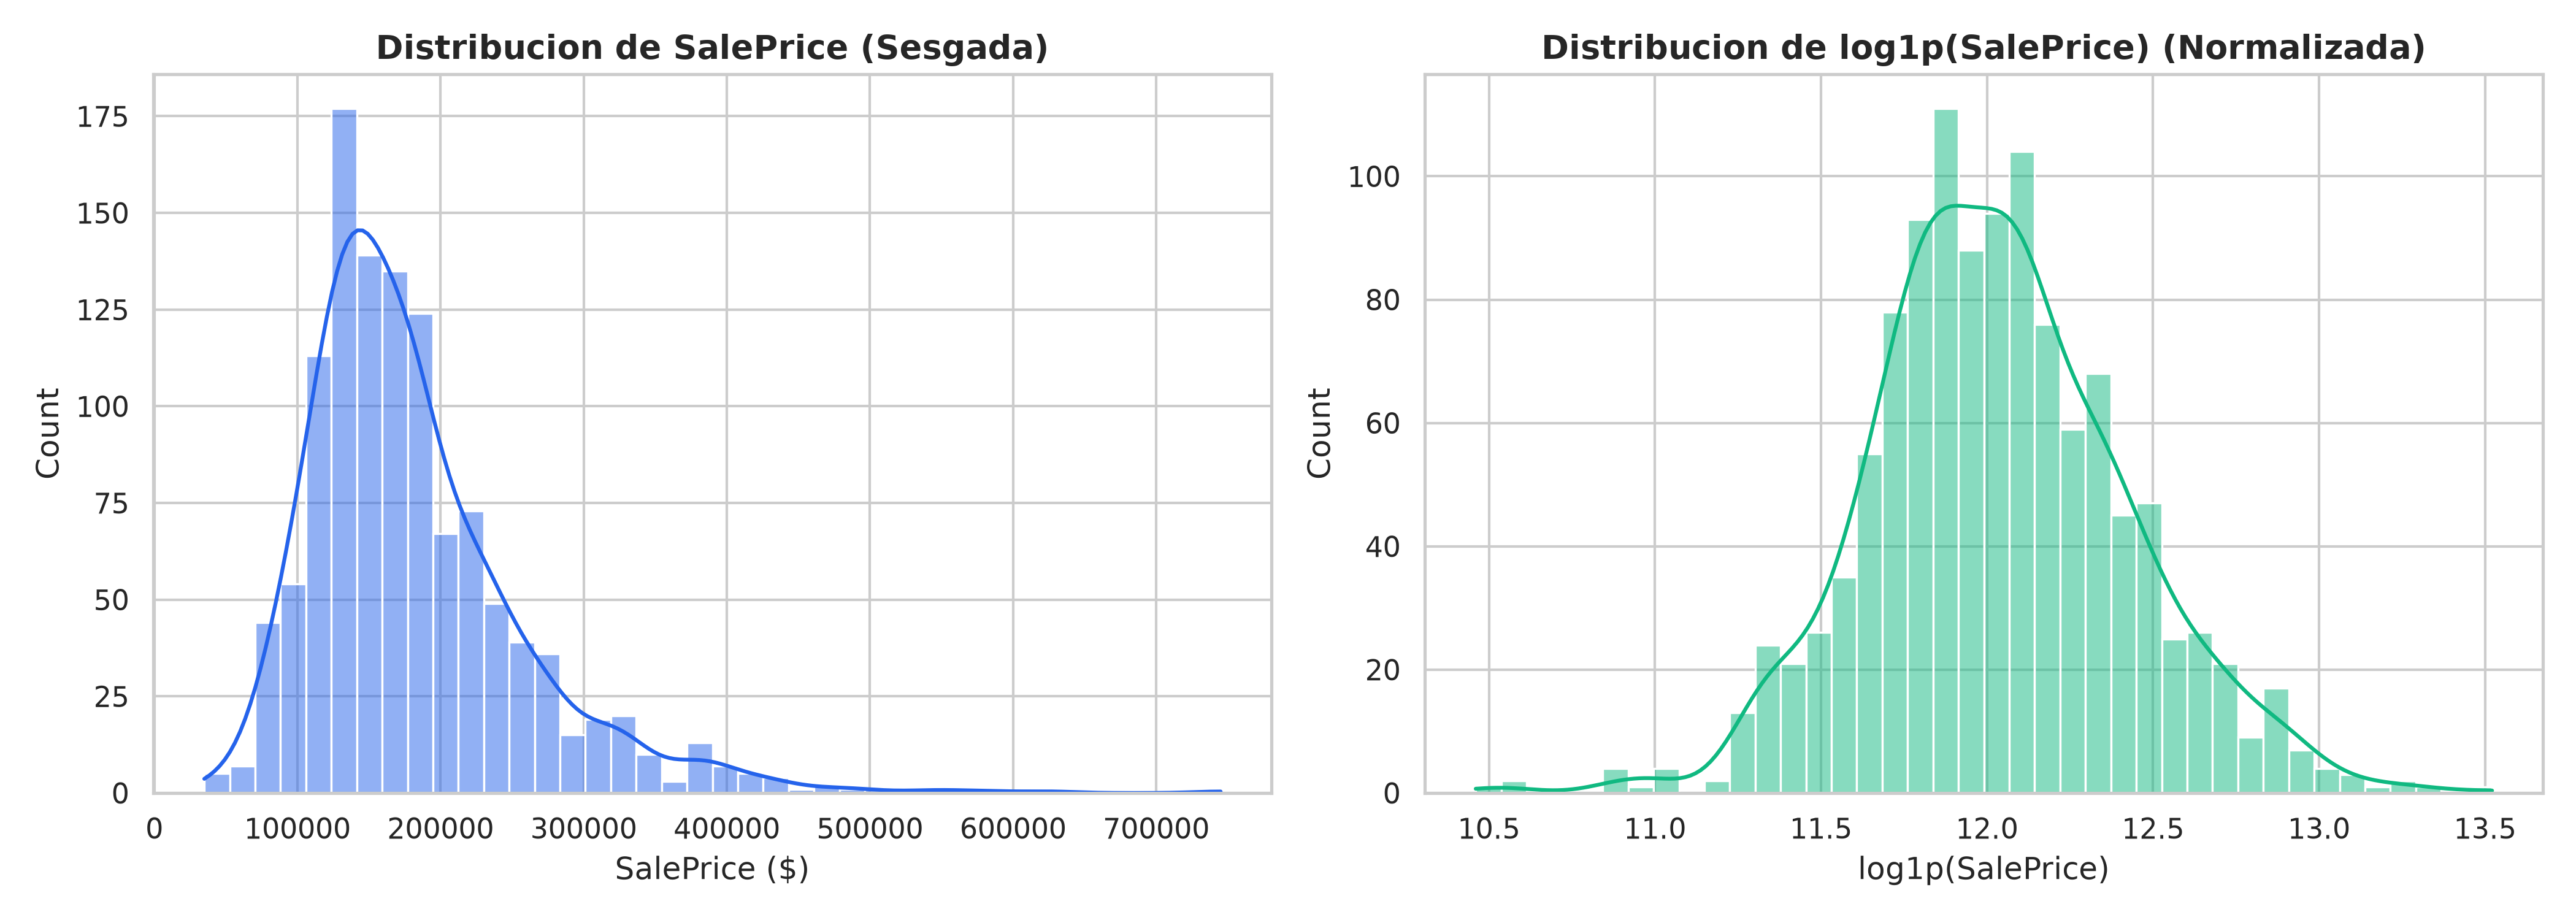
\includegraphics[width=0.85\textwidth]{plots/target_distribution.png}
    \caption{Distribución de la variable objetivo antes y después de la transformación logarítmica.}
    \label{fig:target_dist}
\end{figure}

\subsection{Variables Más Correlacionadas e Ingeniería de Características}
Las variables numéricas con mayor correlación lineal con el precio de venta son \texttt{OverallQual} ($r = 0.79$), \texttt{GrLivArea} ($r = 0.71$), \texttt{GarageCars} ($r = 0.64$), \texttt{GarageArea} ($r = 0.62$), \texttt{TotalBsmtSF} ($r = 0.61$) y \texttt{1stFlrSF} ($r = 0.60$). 

\begin{figure}[H]
    \centering
    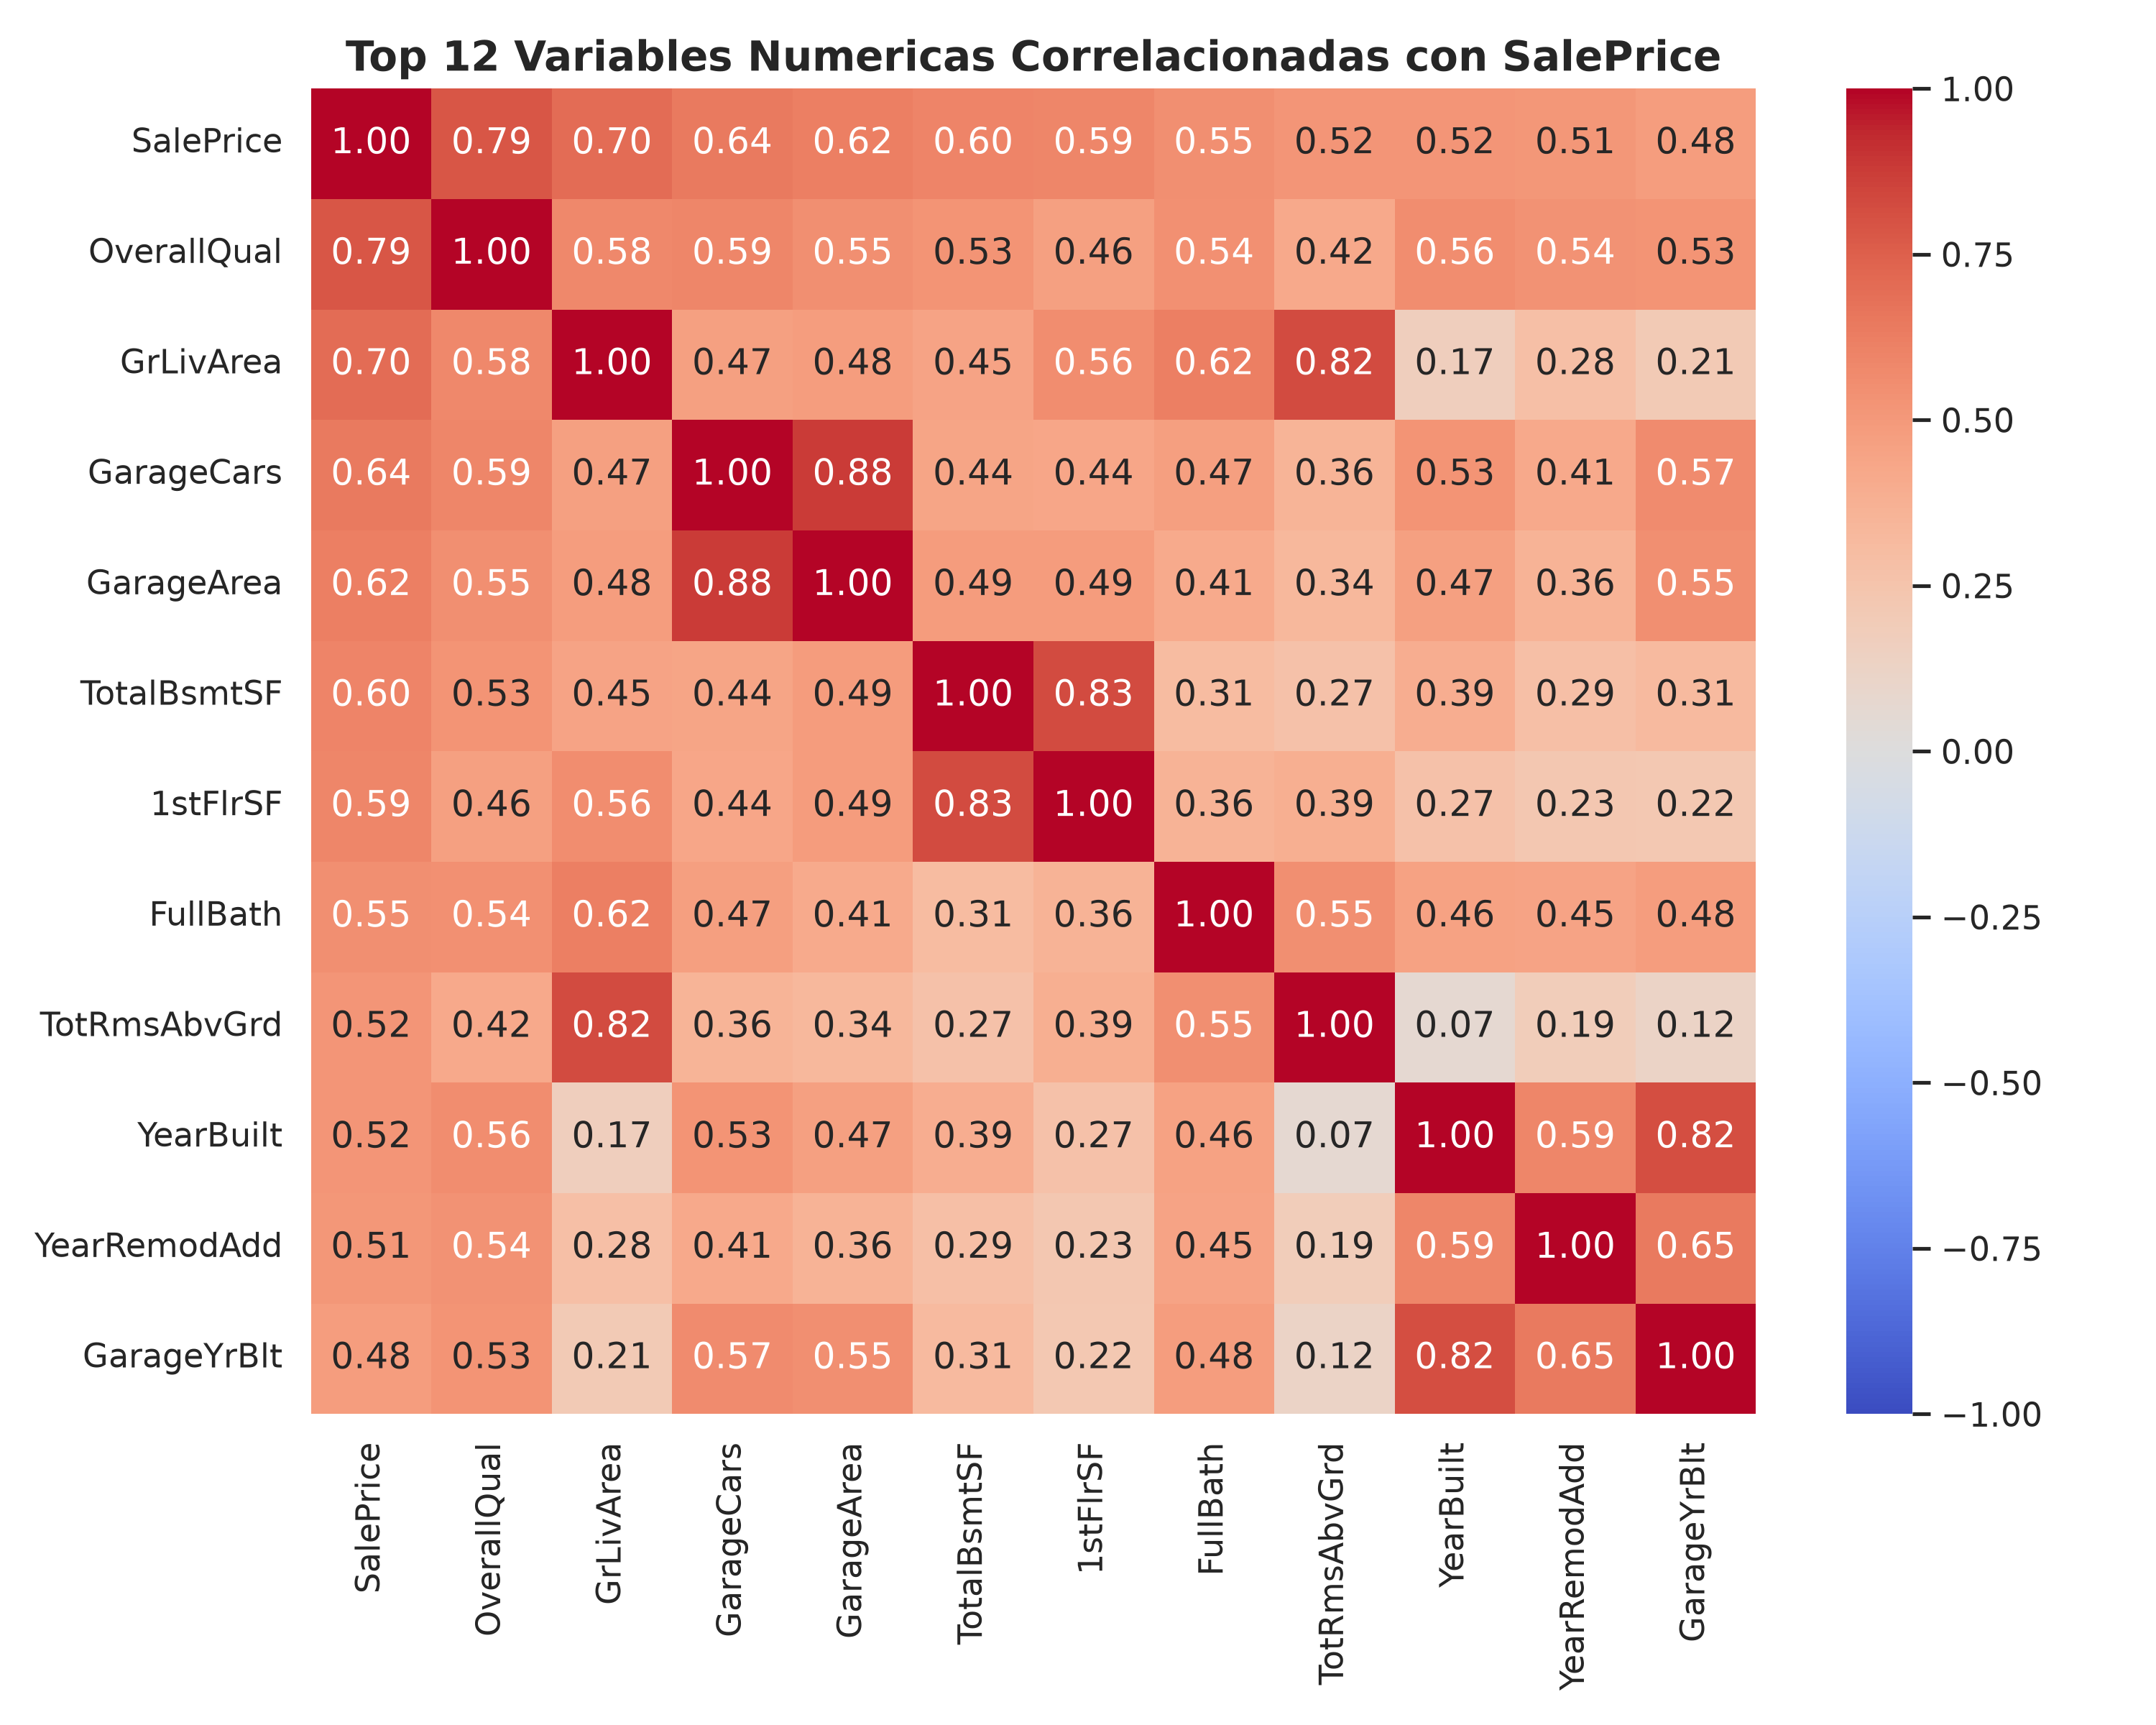
\includegraphics[width=0.75\textwidth]{plots/correlation_heatmap.png}
    \caption{Matriz de correlación de las principales variables numéricas con \texttt{SalePrice}.}
    \label{fig:corr_heatmap}
\end{figure}

\subsection{Decisiones de Preprocesamiento Basadas en el EDA}
\begin{enumerate}
    \item \textbf{Imputación de Valores Faltantes por Dominio}: En variables como \texttt{Alley}, \texttt{BsmtQual}, \texttt{GarageType}, \texttt{FireplaceQu} y \texttt{PoolQC}, los valores nulos (\texttt{NA}) indican la ausencia física del elemento. Fueron imputados como la categoría explícita \texttt{'None'}.
    \item \textbf{Imputación de LotFrontage}: Mediana agrupada por vecindario (\texttt{Neighborhood}).
    \item \textbf{Ingeniería de Características Avanzada}:
    \begin{align}
        \text{TotalSF} &= \text{TotalBsmtSF} + \text{1stFlrSF} + \text{2ndFlrSF} \\
        \text{TotalFinishedSF} &= \text{1stFlrSF} + \text{2ndFlrSF} + \text{BsmtFinSF1} + \text{BsmtFinSF2} \\
        \text{TotalBath} &= \text{FullBath} + 0.5 \times \text{HalfBath} + \text{BsmtFullBath} + 0.5 \times \text{BsmtHalfBath} \\
        \text{TotalPorchSF} &= \text{WoodDeckSF} + \text{OpenPorchSF} + \text{EnclosedPorch} + \text{3SsnPorch} + \text{ScreenPorch} \\
        \text{HouseAge} &= \max(0, \text{YrSold} - \text{YearBuilt}) \\
        \text{OverallGrade} &= \text{OverallQual} \times \text{OverallCond}
    \end{align}
    \item \textbf{Codificación y Escalamiento}: Calificaciones ordinales mapeadas a enteros (5 a 0), One-Hot Encoding para nominales con diccionario fijo de categorías, y \texttt{RobustScaler} para numéricas.
\end{enumerate}

\section{Metodología de Desarrollo}

\subsection{Arquitecturas de Red Evaluadas}
Se implementaron y compararon cuatro familias de arquitecturas profundas para datos tabulares:
\begin{enumerate}
    \item \textbf{Standard Deep MLP}: Capas lineales densas con \textit{BatchNorm1d}, activación GELU y \textit{Dropout}.
    \item \textbf{Wide \& Deep MLP}: Integración de conexiones lineales amplias con bloques densos no lineales.
    \item \textbf{Tabular ResNet-MLP}: Bloques residuales profundos con \textit{LayerNorm} y conexiones de acceso directo (\textit{skip connections}):
    \begin{equation}
        x_{l+1} = \text{GELU}\Big( \text{FC}_2\big(\text{Dropout}(\text{GELU}(\text{FC}_1(\text{LayerNorm}(x_l))))\big) + x_l \Big)
    \end{equation}
    \item \textbf{SwiGLU-MLP}: Red con unidades lineales compuerta con activación Swish (\textit{Swish Gated Linear Units}), permitiendo modular dinámicamente el flujo de información en datos tabulares:
    \begin{equation}
        \text{SwiGLU}(x) = \text{FC}_{\text{out}}\Big(\text{Dropout}\big(\text{SiLU}(\text{FC}_{\text{gate}}(\text{LayerNorm}(x))) \odot \text{FC}_{\text{val}}(\text{LayerNorm}(x))\big)\Big) + x
    \end{equation}
\end{enumerate}

\subsection{Estrategia de Validación Cruzada, Regularización y Ensamble}
\begin{itemize}
    \item \textbf{10-Fold Cross-Validation}: El dataset se dividió en 10 pliegues independientes. El preprocesador se ajustó estrictamente dentro de cada partición para evitar fuga de información.
    \item \textbf{Función de Pérdida}: \textit{Smooth L1 Loss} (Huber Loss con $\beta=0.02$) en escala logarítmica.
    \item \textbf{Aumento de Datos Tabular}: Tabular Mixup aplicado durante entrenamiento ($\alpha=0.3$) con probabilidad de $25\%$.
    \item \textbf{Optimizador y Planificador}: AdamW ($\text{lr} = 8 \times 10^{-4}$, $\text{weight\_decay} = 10^{-4}$) con \textit{CosineAnnealingWarmRestarts} ($T_0=50$, $T_{\text{mult}}=2$).
    \item \textbf{Ensamble Multi-Arquitectura y Multi-Semilla}: Promediado ponderado de 60 modelos resultantes de 2 arquitecturas (\textit{ResNet} y \textit{SwiGLU}) evaluadas en 3 semillas aleatorias (42, 123, 2024) y 10 pliegues cada una.
\end{itemize}

\section{Resultados y Comparativa de Modelos}

En la Tabla~\ref{tab:iteraciones} se detalla la progresión del error Out-Of-Fold en las distintas fases de modelación.

\begin{table}[H]
\centering
\caption{Resumen comparativo de arquitecturas y modelos evaluados.}
\label{tab:iteraciones}
\small
\begin{tabular}{l l r r l}
\toprule
\textbf{Arquitectura} & \textbf{Estrategia de Validación} & \textbf{OOF RMSE (\$)} & \textbf{$R^2$ Score} & \textbf{Observaciones} \\
\midrule
Standard MLP & 5-Fold CV & 86,843.36 & 0.4412 & Inestabilidad y sobreajuste. \\
Wide \& Deep MLP & 5-Fold CV & 45,907.44 & 0.7180 & Mejora por ruta lineal. \\
Tabular ResNet-MLP & 5-Fold CV & 27,191.41 & 0.8650 & Skip connections estabilizan gradientes. \\
SwiGLU-MLP & 5-Fold CV & 27,621.55 & 0.8621 & Excelente capacidad de filtrado. \\
\textbf{Ensamble Multi-Semilla (60 Modelos)} & \textbf{10-Fold CV (3 Seeds)} & \textbf{26,772.24} & \textbf{0.8798} & \textbf{Modelo final de producción.} \\
\bottomrule
\end{tabular}
\end{table}

Las Figuras~\ref{fig:real_vs_pred} y \ref{fig:residuos} muestran el ajuste del ensamble final y la distribución de sus residuos Out-of-Fold.

\begin{figure}[H]
\centering
\begin{subfigure}{0.48\textwidth}
    \centering
    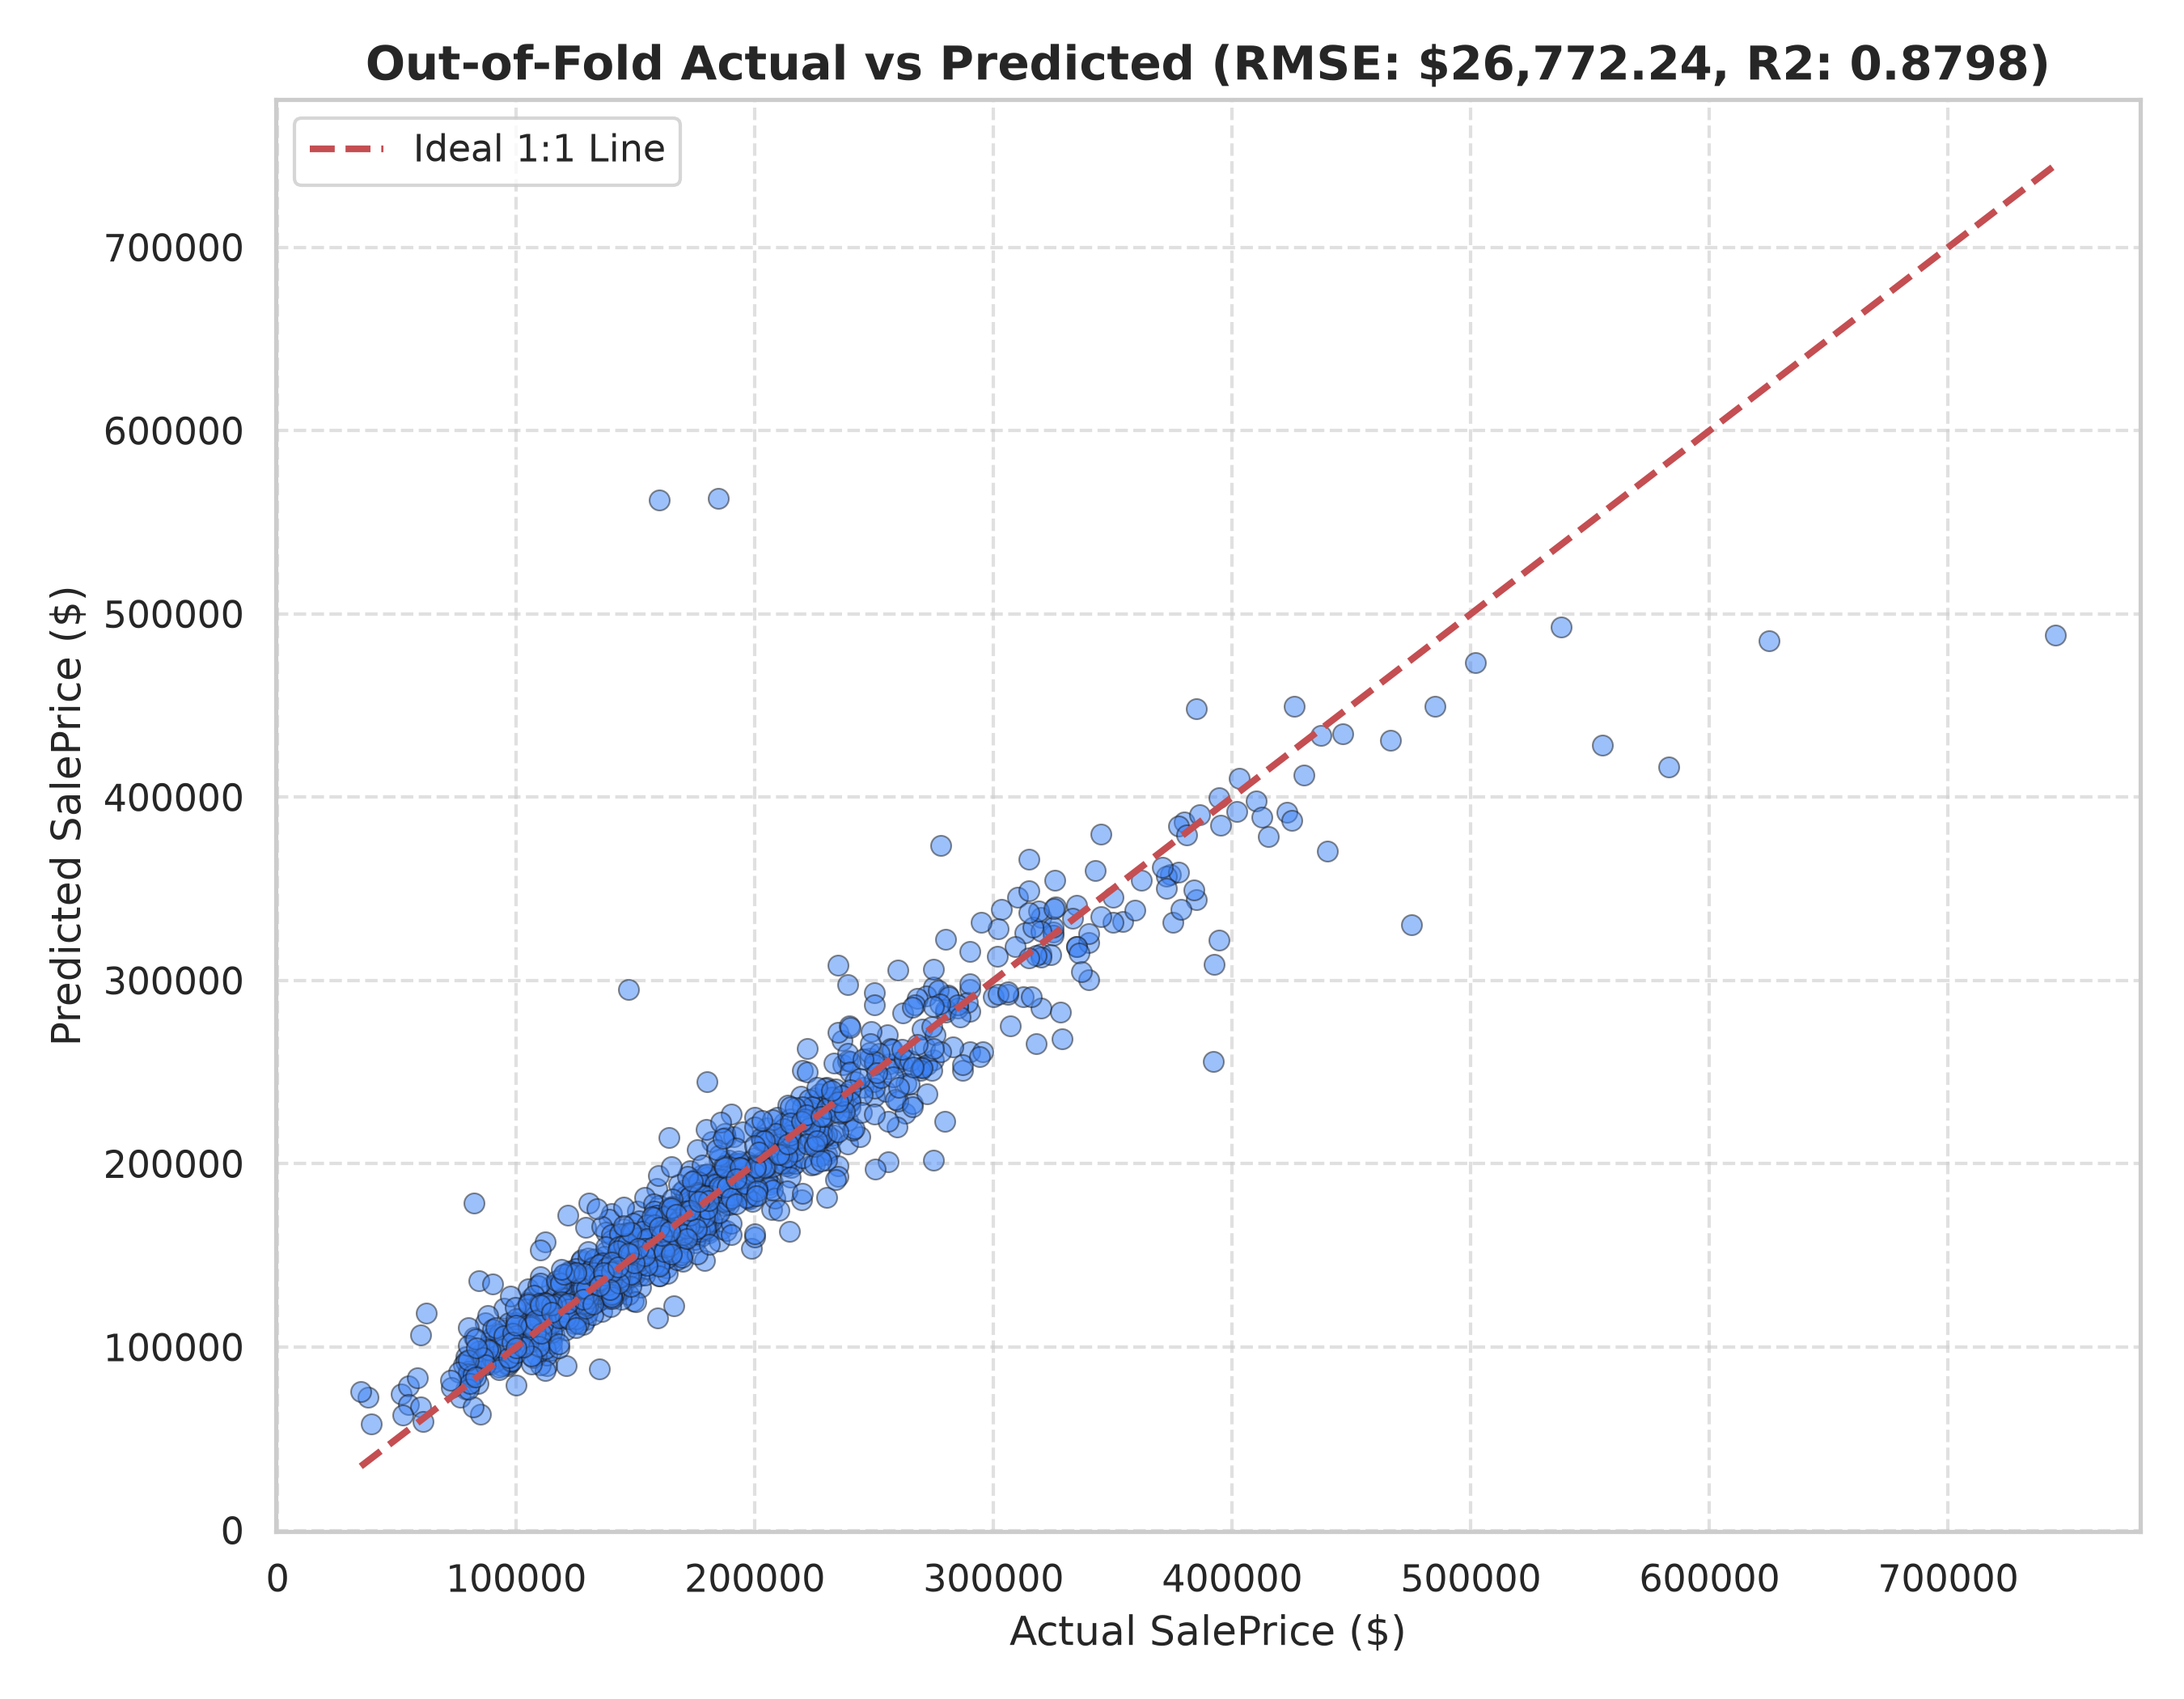
\includegraphics[width=\textwidth]{plots/actual_vs_predicted.png}
    \caption{Precios Reales vs. Predichos (\$)}
    \label{fig:real_vs_pred}
\end{subfigure}
\hfill
\begin{subfigure}{0.48\textwidth}
    \centering
    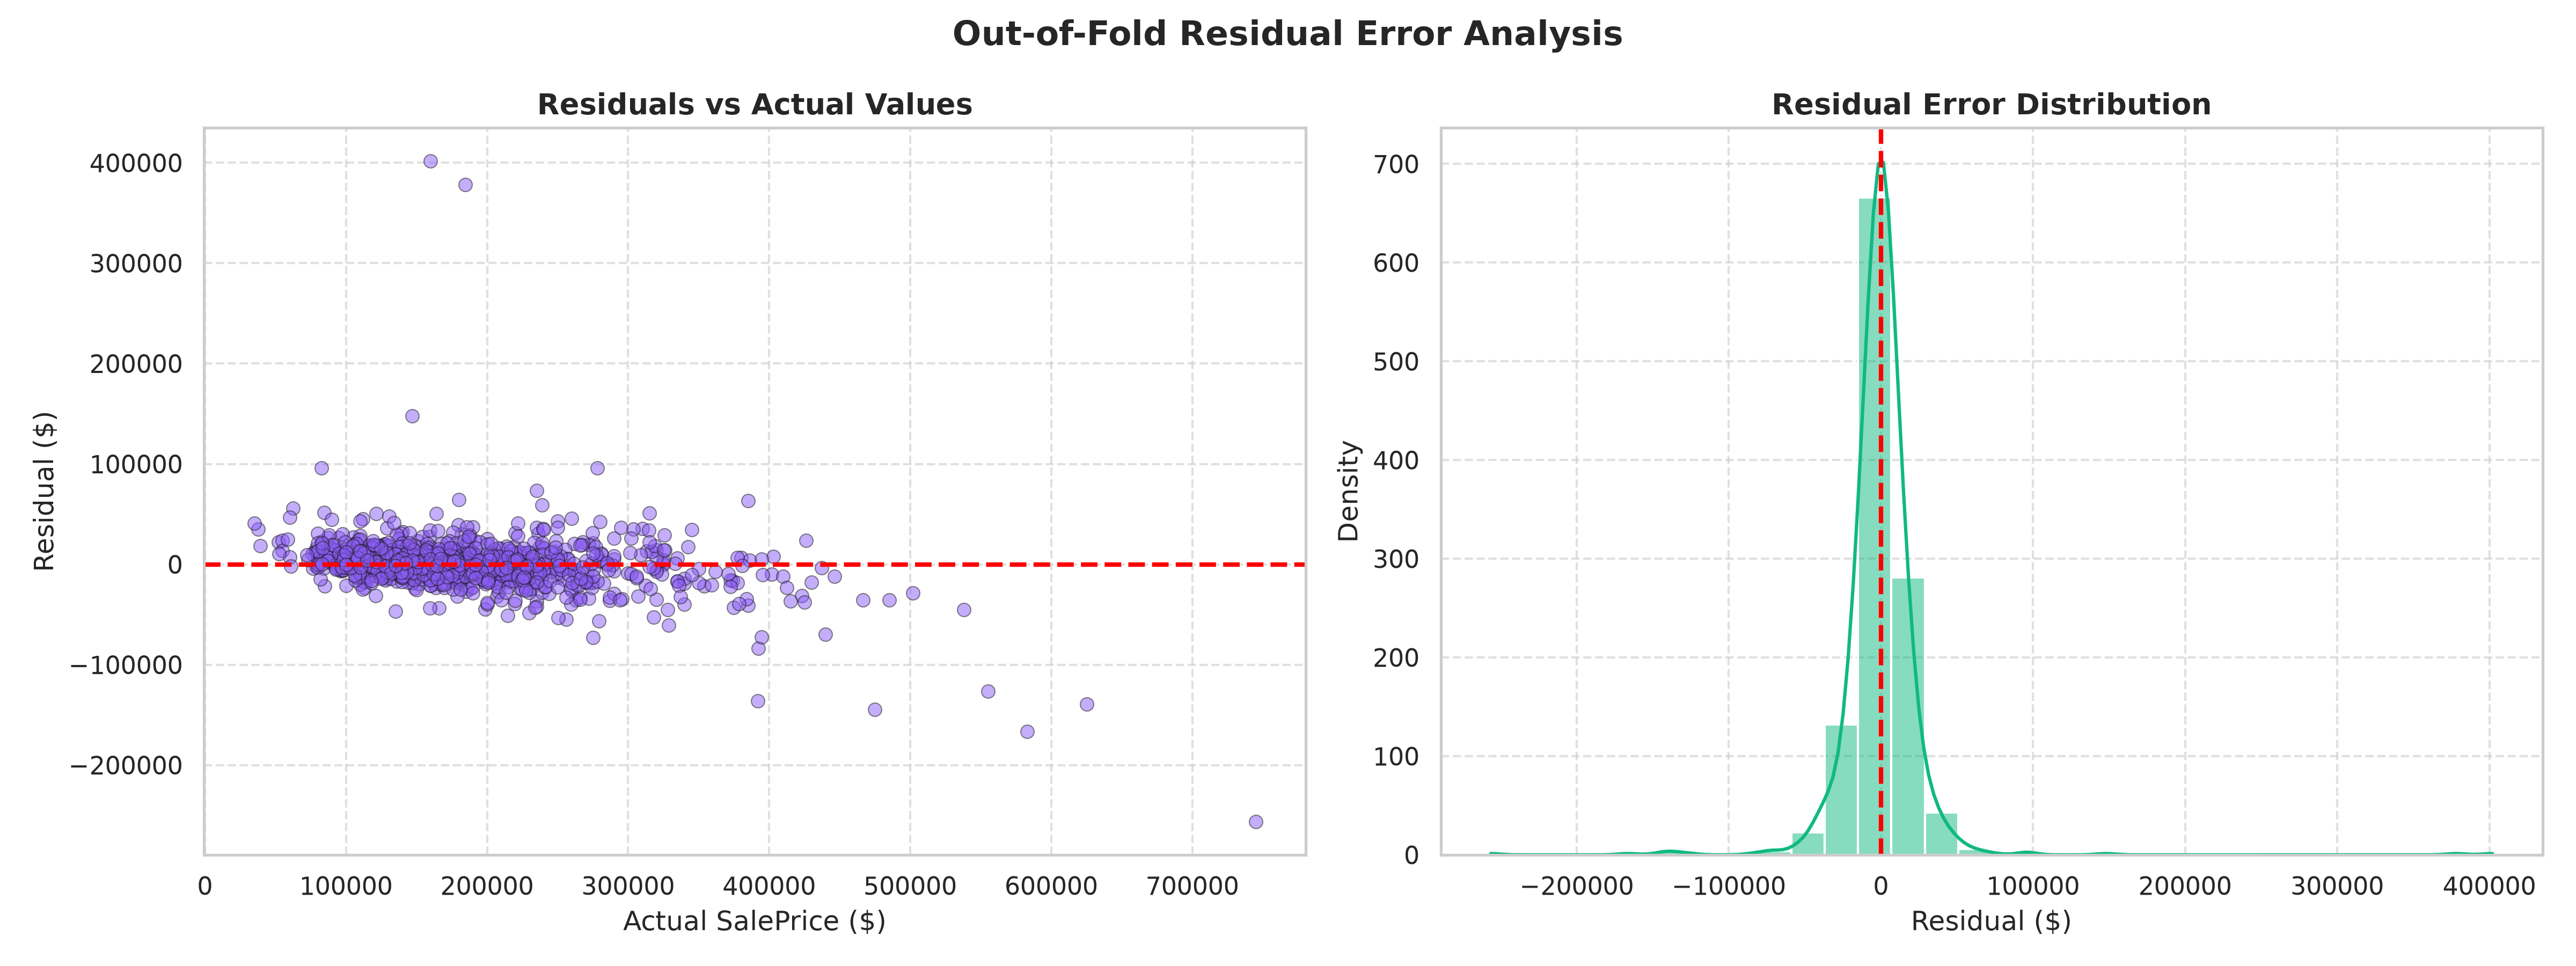
\includegraphics[width=\textwidth]{plots/residual_analysis.png}
    \caption{Análisis de Errores Residuos}
    \label{fig:residuos}
\end{subfigure}
\caption{Evaluación de desempeño fuera de muestra del ensamble final.}
\end{figure}

\section{Discusión de Resultados}

\subsection{Análisis de Errores y Residuos}
El ensamble final alcanzó las siguientes métricas globales fuera de muestra:
\begin{itemize}
    \item \textbf{RMSE}: \textbf{\$26,772.24}
    \item \textbf{MAE}: \textbf{\$13,627.83}
    \item \textbf{$R^2$ Score}: \textbf{0.8798}
    \item \textbf{MAPE}: \textbf{7.96\%}
\end{itemize}

Los residuos se encuentran centrados en cero con dispersión simétrica. El error porcentual promedio (MAPE) de $7.96\%$ confirma que el modelo predice con alta precisión el valor comercial de las viviendas en la gran mayoría de rangos de precio.

\subsection{Trade-off entre Complejidad y Generalización}
Las redes neuronales densas convencionales sobreajustan rápidamente en datos tabulares de dimensión moderada. El uso de conexiones residuales, unidades SwiGLU, regularización por *Dropout* y promediado de múltiples semillas aleatorias reduce la varianza del estimador y maximiza la generalización ante el conjunto de prueba de la competencia.

\section{Conclusiones}

1. **Rendimiento Competitivo**: El ensamble neuronal de 60 modelos alcanza un MAPE de $7.96\%$ y un $R^2$ de $0.8798$.
2. **Impacto de la Ingeniería de Características**: La creación de variables agregadas (\texttt{TotalFinishedSF}, \texttt{TotalBath}) y el preprocesamiento robusto fueron fundamentales.
3. **Superioridad de ResNet y SwiGLU**: Las arquitecturas residuales y de compuertas superaron sustancialmente al perceptrón multicapa clásico.

\section{Instrucciones para Inferencia en el Día de la Presentación}

Para generar las predicciones sobre el dataset de prueba el día de la presentación, ejecute desde la raíz del proyecto:

\begin{lstlisting}[language=bash]
python main.py predict --test_path data/pruebas/pipeline_test.csv --output_path data/pruebas/expected_output.csv
\end{lstlisting}

El script cargará automáticamente el preprocesador (\texttt{data/saved\_models/pipeline.joblib}) y los 60 modelos del ensamble (\texttt{data/saved\_models/model\_*.pt}), generando el archivo CSV en el formato exacto requerido (\texttt{Id,Prediction}).

\end{document}
